\begin{questions}
\question Consider the following sequence of number:
\[\{1, 3, 6, 10, 15, 21, \dots\}.\]
These are called \textit{triangular numbers} because they are the number of vertices as pictured below.
\begin{figure}[hbt!]
\centering
  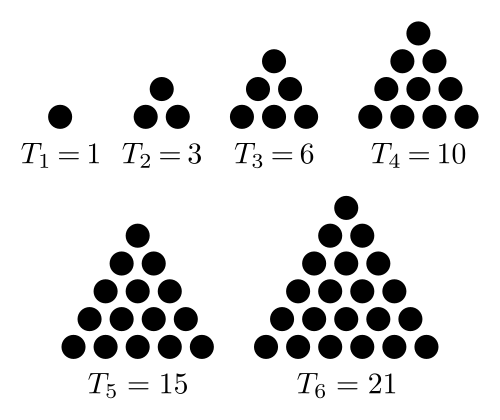
\includegraphics[scale=0.33]{plots/500px_First_six_triangular_numbers.png}
\caption{Triangular Numbers}
\end{figure}
\begin{parts}
  \part Write a \textit{recursive} definition for this sequence.
  \begin{solutionorbox}[0.75in]
    $T_{n+1}=T_n+n+1$ or $T_{n}=T_{n-1}+n$
  \end{solutionorbox}
  
  \part Find an \textit{explicit} formula for this sequence where $n=1$ is the first term of the sequence.
  \begin{solutionorbox}[1.0in]
    By looking at the pattern, we can observe the following:\\
    \begin{center}
      \begin{tabular}{l|l}
        $n$ & $T_n$ \\ \hline
        1   & 1\\
        2   & 1+2\\
        3   & 1+2+3\\
        $\vdots$ & $\vdots$ \\
        $n$ & $\displaystyle 1+2+\dots+n=\sum_{k=1}^n k$
      \end{tabular}
    \end{center}
    The sum of $k$ positive integers is given by the formula: $\frac{n(n+1)}{2}$, so $T_n=\frac{n(n+1)}{2}$.
  \end{solutionorbox}
  
  \part Determine what $T_{100}$ would be.
  \answerline[5050]
\end{parts}

\question Determine if the sequence has a least upper bound (supremum) and a greatest lower bound (infimum). If so, what are they?
\begin{parts}
\part \sequence{e^{-k}}{k=0}{\infty} \answerline[1]
\part \sequence{(-1)^kk}{k=0}{\infty} \answerline[DNE]
\part \sequence{3+\frac{1}{k^2+1}}{k=-\infty}{\infty} \answerline[3]
\end{parts}


\newpage

\question Match the formulas with the descriptions of the behavior of the sequence as $k$ goes to infinity. List the first five values in the sequence as justification of your answer.
\begin{parts}
  \begin{multicols}{3}
    \part \sequence{\frac{(-1)^n}{n+1}}{n=1}{\infty}\\[16pt]
    \part \sequence{\sin\left(\frac{1}{k}\right)}{k=1}{\infty}\\[16pt]
    \part \sequence{-4+\frac{(-1)^m}{m}}{m=0}{\infty}\\[16pt]
    \part \sequence{\frac{n\cos(n)}{2n+3}}{n=12}{\infty}\\[16pt]
    \part \sequence{n(n-1)-n}{n=-2}{\infty}\\[16pt]
    \part \sequence{-\frac{p!}{(p+1)!}}{p=0}{\infty}\\[16pt]
  \end{multicols}
\end{parts}

\begin{enumerate}[I.]
\item \numanswerline[D] Converges to $\frac{1}{2}$ from above and below.\vfill

\item \numanswerline[A] Converges to $0$ through positive numbers.\vfill

\item \numanswerline[B] Converges to $0$ from above and below.\vfill

\item \numanswerline[F] Converges to 0 through negative numbers.\vfill

\item \numanswerline[E] Diverges to $\infty$.\vfill

\item \numanswerline[C] Converges to $-4$ from above and below.\vfill
\end{enumerate}

\newpage

\question Opiates are drugs with a ``morphine-like pharmacological action" according to the Mayo Clinic \footnote{\url{https://www.mayomedicallaboratories.com/test-info/drug-book/opiates.html}}. Many of these drugs have a half-life of about 5 hours. Suppose a pharmaceutical company has developed a new synthetic opiate with a half-life of 6 hours.
\begin{parts}
\part Complete the following table to describe the first 24 hours after taking 20mg of the new synthetic opiate at 6 hour intervals.

\begin{table}[hbt!]\centering
  \begin{tabular}{l|c|c|c|c|c}
    hour           & 0 & 6 & 12 & 18 & 24 \\ \hline
    amount (mg)    & \myspace & \myspace & \myspace & \myspace & \myspace
  \end{tabular}
\end{table}

\begin{solution}
  \begin{center}
    \begin{tabular}{l|c|c|c|c|c}
      hour           & 0 & 6 & 12 & 18 & 24 \\ \hline
      amount (mg)    & 20 & 10 & 5 & 2.5 & 1.25
    \end{tabular}
  \end{center}
\end{solution}\vfill

\part Write an explicit equation that models this data of the form $N(t)=a_0(r)^{kt}$.
\begin{solutionorbox}[2.25in]
  $N(t)=20\left(\frac{1}{2}\right)^{t/6}=20\left(\sqrt[6]{\frac{1}{2}}\right)^{t}$
\end{solutionorbox}\vfill

\part What is the hourly decay rate of the drug?
\answerline[About 11\%]\vfill
\textit{}
\part As $t\to\infty$, what happens to the amount opiates?
\begin{solutionorlines}[1in]
The amount will tend towards zero.
\end{solutionorlines}\vfill


\end{parts}

\newpage

\question In this question, you will look at a sequence of functions, rather than a numerical sequence. Consider the function defined by $f_n(x)=\left(1+\frac{x}{n}\right)^n$ and the sequence defined by \sequence{f_n(x)}{n=0}{\infty}. Go to \url{https://www.desmos.com/calculator/wjwfifwfnn} to help with this question.
\begin{parts}
\part Below are the first 5 terms of this sequence of functions:
\[1\]
\[x+1\]
\[\frac{1}{4} x^{2} + x + 1\]
\[\frac{1}{27} x^{3} + \frac{1}{3} x^{2} + x + 1\]
\[\frac{1}{256} \, x^{4} + \frac{1}{16} \, x^{3} + \frac{3}{8} \, x^{2} + x + 1\]
What patterns or sequences of numbers do you notice?
\begin{solutionorbox}[1.75in]
  Answers will vary greatly. One possible answer is the fact that the leading coefficients (assuming $n\geq1$) is $n^n$.
\end{solutionorbox}\vfill

\part Use the Desmos graph that has been provided to record the different values of $f_n(1)$ to four decimal places.
\begin{table}[hbt!]\centering
  \begin{tabular}{c|c|c|c|c|c|c}
    $n$           & 0 & 1 & 10 & 100 & 1000 & $\infty$ \\ \hline
    $f_n(1)$    & \myspace & \myspace & \myspace & \myspace & \myspace & \myspace\\ \hline
    $f_n(2)$    & \myspace & \myspace & \myspace & \myspace & \myspace & \myspace
  \end{tabular}
\end{table}

\begin{solution}
\begin{center}
  \begin{tabular}{c|c|c|c|c|c|c}
    $n$           & 0 & 1 & 10 & 100 & 1000 & $\infty$ \\ \hline
    $f_n(1)$    & DNE & 2 & 2.594 & 2.705 & 2.171 & e \\ \hline
    $f_n(2)$    & DNE & 3 & 6.1717 & 7.2446 & 7.3743 & $e^2$
  \end{tabular}
\end{center}
\end{solution}


\vfill

\part What function do you hypothesize this sequence of functions converges to as $n\to\infty$? Give a justification of your answer. [Hint: $\lim_{n\to\infty}(1+1/n)^{n}=e$]
\begin{solutionorbox}[1.75in]
\[e^x\]
\end{solutionorbox}

\end{parts}

\newpage

\question Determine if the sequence is bounded or unbounded, then use an appropriate test to analyze the monotonicity of the given sequence.
\begin{parts}
\part \sequence{\frac{n}{n+3}}{n=0}{\infty}
\begin{solutionorbox}[2.5in]
We can use the Difference Test to show that this series is strictly increasing. 
\[\begin{aligned}
  a_{n+1}-a_n   &=\frac{n+1}{n+4}-\frac{n}{n+3} \\
                &=\frac{(n+1)(n+3)-n(n+4)}{(n+4)(n+3)} \\
                &=\frac{3}{(n+3)(n+4)}
\end{aligned}\]
So, $\forall_{n\geq0}a_{n+1}-a_n>0$; therefore, this sequence is strictly increasing. It is bounded below by 0 and above by 1.
\end{solutionorbox}

\part \sequence{\frac{k^3}{(k-1)!}}{k=0}{\infty}
\begin{solutionorbox}[2.5in]
Since we have a factorial in the problem, we should use the Ratio Test to determine the monotonicity. So, consider $\frac{a_{k+1}}{a_k}$.
\[\begin{aligned}
  \frac{a_{n+1}}{a_n}   &=\frac{(k+1)^3}{k!}\cdot\frac{(k-1)!}{k^3} \\
                        &=\frac{(k+1)^3}{k\cancel{(k-1)!}}\cdot\frac{\cancel{(k-1)!}}{k^3} \\
                        &=\frac{(k+1)^3}{k^4}
\end{aligned}\]
From this, we see that that this is converging to zero, which means it will be less than 1. However, it isn't less than 1 until $k\geq3$. Therefore, this sequence is eventually decreasing, bounded below by zero, and abounded above by 13.5.
\end{solutionorbox}

\part \sequence{e^{-k}k^3}{k=0}{\infty}
\begin{solutionorbox}[2.5in]
We'll use the First Derivative Test to show this is decreasing. First, we make the sequence continuous by making the function $a(x)=e^{-x}x^3$. Now, we take the derivative of $a(x)$: $a'(x)=x^2e^{-x}(3-x)$. Now, we'll create the sign chart.\\[4pt]

\begin{center}
\begin{tikzpicture}[]
  \draw[latex-latex,color=firstDerivative,line width=0.6mm] (-1,0)--(5,0); %edit for axis
  \foreach \x in  {0,3} % edit here for the vertical lines
  \draw[shift={(\x,0)},color=black] (0pt,3pt) -- (0pt,-3pt);
  \foreach \x in {0,3} % edit here for the numbers
  \draw[shift={(\x,0)},color=black] (0pt,0pt) -- (0pt,-3pt) node[below] {$\x$};
  
  %Insert Signs
  \node at (5.5,0pt) {$a'(x)$};
  \node at (1.5, 0.33) {$+$};
  \node at (4, 0.33) {$-$};
\end{tikzpicture}
\end{center}

So, $\forall_{x>3}a'(x)<0$, which means that $a(x)$ is decreasing after $x=3$. This, in return, means that the sequence is eventually decreasing, bounded above by $27e^{-3}$, and bounded below by 0.
\end{solutionorbox}
\end{parts}

\end{questions}